\documentclass{sigchi}

% Use this command to override the default ACM copyright statement (e.g. for preprints). 
% Consult the conference website for the camera-ready copyright statement.


%% EXAMPLE BEGIN -- HOW TO OVERRIDE THE DEFAULT COPYRIGHT STRIP -- (July 22, 2013 - Paul Baumann)
% \toappear{Permission to make digital or hard copies of all or part of this work for personal or classroom use is 	granted without fee provided that copies are not made or distributed for profit or commercial advantage and that copies bear this notice and the full citation on the first page. Copyrights for components of this work owned by others than ACM must be honored. Abstracting with credit is permitted. To copy otherwise, or republish, to post on servers or to redistribute to lists, requires prior specific permission and/or a fee. Request permissions from permissions@acm.org. \\\textbf{}
% {\emph{CHI'14}}, April 26--May 1, 2014, Toronto, Canada. \\
% Copyright \copyright~2014 ACM ISBN/14/04...\$15.00. \\
% DOI string from ACM form confirmation}
%% EXAMPLE END -- HOW TO OVERRIDE THE DEFAULT COPYRIGHT STRIP -- (July 22, 2013 - Paul Baumann)
\toappear{Permission to make digital or hard copies of part or all of this work for personal or classroom use is granted without fee provided that copies are not made or distributed for profit or commercial advantage and that copies bear this notice and the full citation on the first page. Copyrights for third-party components of this work must be honored. For all other uses, contact the owner/author(s). Copyright is held by the author/owner(s).\\
{\emph{SUI'14}}, October 4–5, 2014, Honolulu, HI, USA.\\
ACM 978-1-4503-2820-3/14/10.\\
\changes{TODO: DOI string goes here.}}

% Arabic page numbers for submission. 
% Remove this line to eliminate page numbers for the camera ready copy
%\pagenumbering{arabic}


% Load basic packages
\usepackage{balance}  % to better equalize the last page
\usepackage{graphics} % for EPS, load graphicx instead
\usepackage{times}    % comment if you want LaTeX's default font
\usepackage{url}      % llt: nicely formatted URLs
% llt: Define a global style for URLs, rather that the default one
\makeatletter
\def\url@leostyle{%
  \@ifundefined{selectfont}{\def\UrlFont{\sf}}{\def\UrlFont{\small\bf\ttfamily}}}
\makeatother
\urlstyle{leo}

\usepackage{gensymb}
\usepackage{afterpage}
% see http://tex.stackexchange.com/questions/46055/typesetting-with-inch-symbols-and-sizes-in-inches
% \usepackage{mathpazo}
\usepackage{amsmath}
\def\inch#1{#1''}
\def\ft#1{#1'\thinspace}



% comment macros are in inputmacros.tex
% set up tight list spacing
\usepackage{enumitem} 
\setlist{nolistsep,nosep}

% for toggles
\usepackage{etoolbox}

\newcommand {\studyquote}[1]{\em ``#1''\normalfont}

% CHANGE FROM TOGGLE TRUE TO TOGGLE FALSE FOR NON-ANONYMOUS RENDERING
% http://tex.stackexchange.com/questions/5894/latex-conditional-expression
\newtoggle{anonymous}
%\togglefalse{anonymous}
\toggletrue{anonymous}

% CHANGE FROM TOGGLE TRUE TO TOGGLE FALSE TO HIDE COMMENTS
\newtoggle{comments}
%\toggletrue{comments}
\togglefalse{comments}

% Comment region command (from Wesley Willett)
\usepackage[usenames]{color}
\usepackage[usenames,dvipsnames]{xcolor}
\iftoggle{comments} {
  %if we want to show comments
  \newcommand {\claire}[1]{{\color{Orange}\bf{CT: #1}\normalfont}}
  \newcommand {\sean}[1]{{\color{BlueGreen}\bf{SC: #1}\normalfont}}
  \newcommand {\yang}[1]{{\color{NavyBlue}\bf{YL: #1}\normalfont}}
  \newcommand {\ben}[1]{{\color{violet}\bf{BZ: #1}\normalfont}}
  \newcommand {\bjoern}[1]{{\color{BrickRed}\bf{BH: #1}\normalfont}}
  \newcommand {\achal}[1]{{\color{OliveGreen}\bf{AD: #1}\normalfont}} % can't find another color...
  \newcommand {\changes}[1]{{\color{Red}\bf{#1}\normalfont}}
}{
  %if we don't want to show comments
  \newcommand {\claire}[1]{}
  \newcommand {\sean}[1]{}
  \newcommand {\yang}[1]{}
  \newcommand {\ben}[1]{}
  \newcommand {\bjoern}[1]{}
  \newcommand {\achal}[1]{}
  \newcommand {\changes}[1]{{#1}}
}
\newcommand {\systemname}{HOBS }
\newcommand {\systemnamenospace}{HOBS}

% To make various LaTeX processors do the right thing with page size.
\def\pprw{8.5in}
\def\pprh{11in}
\special{papersize=\pprw,\pprh}
\setlength{\paperwidth}{\pprw}
\setlength{\paperheight}{\pprh}
\setlength{\pdfpagewidth}{\pprw}
\setlength{\pdfpageheight}{\pprh}

% Make sure hyperref comes last of your loaded packages, 
% to give it a fighting chance of not being over-written, 
% since its job is to redefine many LaTeX commands.
\usepackage[pdftex]{hyperref}
\hypersetup{
pdftitle={SIGCHI Conference Proceedings Format},
pdfauthor={LaTeX},
pdfkeywords={SIGCHI, proceedings, archival format},
bookmarksnumbered,
pdfstartview={FitH},
colorlinks,
citecolor=black,
filecolor=black,
linkcolor=black,
urlcolor=black,
breaklinks=true,
}

% create a shortcut to typeset table headings
\newcommand\tabhead[1]{\small\textbf{#1}}


% End of preamble. Here it comes the document.
\begin{document}


% as we discussed last time, the "Sees" and "Line-of-sight" suggests some computer vision direction 
% need a different title for sure, but not in a hurry
\title{\systemnamenospace: Head Orientation Based Selection\\in Physical Spaces}
%Project GlasSees: Direct Interaction Through Line-of-sight}

\iftoggle{anonymous}{
\author{
 \alignauthor Anonymous for submission\\
    %\affaddr{...}\\
    %\email{...}\\
  }
}{ %else
  \numberofauthors{1}
  \author{
  \alignauthor  Ben Zhang$^{\dagger}$, Yu-Hsiang Chen$^{\dagger}$, Claire Tuna$^{\dagger}$, Achal Dave$^{\dagger}$,\\Yang Li$^{\ddagger}$, Edward Lee$^{\dagger}$, Bj\"orn Hartmann$^{\dagger}$ \\
  \affaddr{$\dagger$: UC Berkeley EECS \& CITRIS Invention Lab \hspace{0.25in} $\ddagger$: Google Research}\\
  \email{\{benzh,clairetuna,achal,eal,bjoern\}@berkeley.edu, sean.yhc@gmail.com, yangli@acm.org}
  }
}

\teaser{
  \centering
  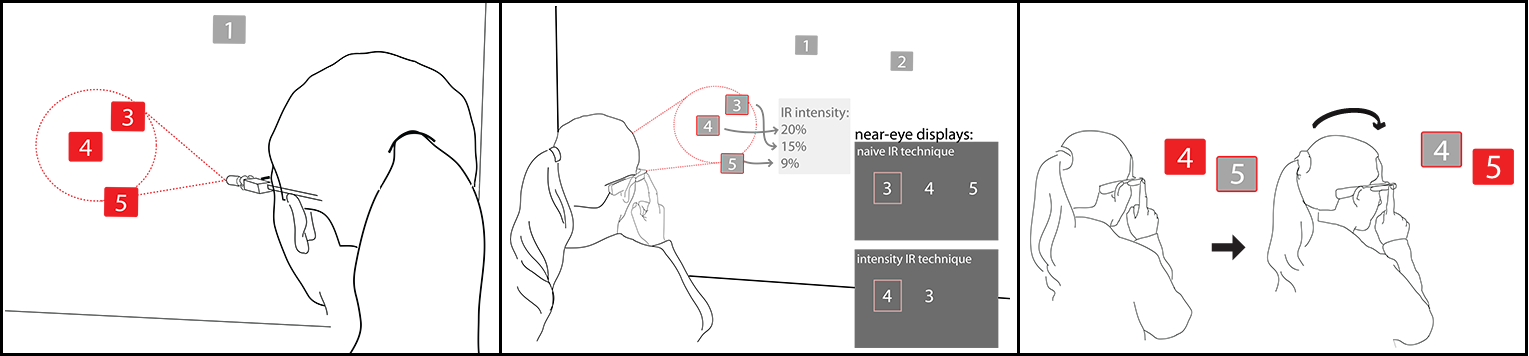
\includegraphics[width=\textwidth]{figures/teaser.png}
  \caption{{\em Left}: Our head orientation-based selection techniques use an IR emitter -- multiple targets may fall within its illumination area. {\em Center}: We offer two list-based refinement techniques -- {\em Naive IR} uses alphabetical ordering; {\em Intensity IR} orders targets by IR intensity. {\em Right}: Using {\em Head-motion Refinement} technique, users can refine their selection through head orientation refinement in a quasi-mode when they hold the touchpad.}
  \label{fig:teaser}
}

%% the third part of the teaser: An example application of head-orientation targeting: Using an augmented head-worn device (1), users can control smart home appliances (2) by looking at them. A near-eye display then shows an appliance control UI (3), which users navigate through multitouch gestures.}

\maketitle

\begin{abstract}
%!TEX root = uist14.tex

%% Yang suggests: Interacting with smart objects in the physical space efficiently is a realistic challenge as these objects become ubiquitous. In this paper, we contribute HOBS, a set of novel methods for selecting physical objects at a distance using infrared-sensed head orientations. We augment a commercial head-worn device, Google Glass, with an infrared (IR) emitter to select targets equipped with IR receivers. We present the iterative design process of our methods, involving a series of interaction technique and hardware design and user evaluations....
Emerging head-worn computing devices can enable interactions with smart objects in physical spaces.
%
We present the iterative design and evaluation of \systemname -- a Head-Orientation Based Selection technique for interacting with these devices at a distance. We augment a commercial wearable device, Google Glass, with an infrared (IR) emitter to select targets equipped with IR receivers. Our first design shows that a naive IR implementation can outperform list selection, but has poor performance when refinement between multiple targets is needed. A second design uses IR intensity measurement at targets to improve refinement. To address the lack of natural mapping of on-screen target lists to spatial target location, our third design infers a spatial data structure of the targets enabling a natural head-motion based disambiguation.
%
Finally, we demonstrate a universal remote control application using HOBS and report qualitative user impressions.

\end{abstract}
\vspace{-0.05in}
\keywords{
  Wearable computing; spatial interaction; selection; Glass%; infrared
}
\vspace{-0.1in}
%% refer to http://www.acm.org/about/class/ccs98-html
\category{H.5.2.}{Information Interfaces and Presentation (e.g. HCI)}{Interaction styles}% (e.g., commands, menus, forms, direct manipulation).}

%!TEX root = sui14.tex
\vfill
\section{Introduction}
%\bjoern{We should see if we can change language in a few places to strengthen the connection to ``Spatial User Interaction", the title of the conference.}

%% from the swarm vision to the necessity of selection
The number of smart objects in our environment with embedded computation and communication has grown rapidly. These objects are all potential targets for interaction. To initiate {\em spatial interactions}, a user needs to first acquire the target object -- a fundamental task that has been extensively studied in graphical user interfaces, but not yet well-explored in {\em physical spaces}.

\changes{Today, companies like Samsung and Whirlpool are making smart appliances with companion applications that use smartphones as {\em universal remote controls}. With these applications, the user can select a device from a list in order to control it with a device-specific user interface. However, this method faces {\em naming} issues (i.e. ``what do we name the lamp on the left?'') and {\em scaling} issues as the number of controlled devices increases. These solutions also present a necessarily flawed mapping from the positions of the appliances in the rich, 3-dimensional world to their place in a 1D or 2D list presented on the screen. }
%
%% previous approaches are limited
Past research has used direct aiming at target devices in space with phones to overcome these problems~\cite{beigl_point_1999,patel_2-way_2003}. Such techniques have a few drawbacks: the aiming device first has to be retrieved; the user's hands have to be free for operation; and the user's visual attention is split between looking down at a screen and out at targets in the world. 

%% introducing head-worn computing and head orientation
Emerging head-worn computing devices do not require retrieval since the devices are already worn; they may enable hands-free or uni-manual interactions; and they offer near-eye or see-through displays to present information in the wearer's field of view. We thus investigate how such computing devices may be used for the selection and control of devices in physical spaces. Head-worn devices can naturally exploit the user's head orientation, an important (but imprecise) indicator of the user's {\em locus of attention}~\cite{raskin}. It suggests the general direction, but not the particular point of focus. We draw an analogy to assistive area cursors and adapt area cursor techniques~\cite{kabbash1995prince,worden1997making,findlater2010enhanced} for physical selection. Such techniques employ a two-step selection process: a {\em coarse} selection of an area of interest, followed by a {\em refinement} to select a target within that area.

In this paper, we describe the iterative development and evaluation of \systemnamenospace, an area-selection technique that can be readily implemented with small hardware changes to emerging head-worn devices. We augment Google Glass\footnote{\url{http://www.google.com/glass/start/}} to enable infrared (IR) communication between Glass and target appliances. We contribute and evaluate new methods for addressing selection ambiguity in this context. In all our techniques, the emitted IR beam %(a diameter of 30-60cm and distance up to 8m)%
 provides an initial {\em coarse} selection area (illustrated in Figure~\ref{fig:teaser} {\em left}). To {\em refine} selection when multiple targets have received IR signals, we describe and evaluate three techniques:

 Our {\em Naive IR} technique shows an alphabetically ordered disambiguation list on the near-eye display (Figure~\ref{fig:teaser} center). A study with $14$ participants finds that target acquisition with naive IR targeting is preferred by users and is faster than pure list selection without IR, but refinement is still time consuming.

Our {\em Intensity IR} technique improves refinement as target objects compare IR received signal strength (RSS). This value allows the system to eliminate some peripheral targets and to re-order the refinement interface's list by their intensity values. For example, in Figure~\ref{fig:teaser} of {\em Intensity IR} technique, device 5 is eliminated first and the list is re-ordered based on the intensity readings. A second study with $10$ participants shows that {\em Intensity IR} successfully reduces both the probability of needing to do refinement as well as the time spent in list navigation when compared to {\em Naive IR}.

Our final {\em Head-motion Refinement} addresses the lack of a natural mapping when users select a target in the refinement step using their device's touchpad --- the axes of motion do not map directly to the spatial layout of target devices in a room. We first learn the relative spatial structure of the targets using Glass' orientation sensors. Users can then perform head movements to change selections to spatially adjacent targets (see the right of Figure~\ref{fig:teaser}). For example, nodding down to select the target below current selection, or tilting right to select the next target on the right. We present preliminary feedback from participants on this technique.

We also demonstrate an example application of our technique used as a remote control of smart appliances such as lighting and TV sets: a user looks at the appliance he wishes to control and confirms selection by tapping. An appliance-specific user interface is then shown on the user's near-eye display for further interactions. 

%Orientation-based selection enables a wide range of context-aware applications. Examples include smart home remote control, break reminder monitor starer, museum attention tracking, indoor positioning, etc. In Figure\,\ref{fig:teaser}, it's a demonstration of the ``universal remote control'' scenario. The user can easily select the smart appliances by simply looking at it's general direction and confirm such selection with either voice command or by tapping the Glass input pad. Then an appliance-specific control UI will be shown on the head-mounted display. For this application, we have asked 14 participants to try the system and we report the qualitative results from them performing home automation tasks.


% In summary, this paper makes the following contributions:
% \begin{itemize}
% \item We presented our three iteractions of design.
% \item We present evaluations that compare head orientation targeting to list selection and quantify the benefits of automatic disambiguation.
% \item We demonstrate a home appliance remote control application built on top of our selection technique.
% \end{itemize}



%%% Local Variables: 
%%% mode: latex
%%% TeX-master: "sui14"
%%% End: 

%!TEX root = sui14.tex
\section{Background and Related Work}
Our approach is related to head- and eye-controlled interfaces, area cursors and prior work on hardware devices for pointing in physical spaces.

\vfill
\ben{make sure no section title appears at the end of any column.}
\subsection{Head and Gaze Input}
\changes{Head movement has long been used for virtual camera control in VR applications~\cite{pausch_user_1993} and as an assistive input technology for cursor control of desktop applications~\cite{radwin1990method}. However, it is notable that human neck muscles have a lower bandwidth than other muscle groups, e.g., the wrist~\cite{card_morphological_1991}.}
%
%Card, summarizing other work, shows that neck muscles are a poor muscle group for pointing in general: neck muscles only have a bandwidth of about $4.2bits/s$ (compared to $23bits/s$ of wrist muscles used by a standard mouse~\cite{Card:1991:MAD:123078.128726}. 
%
Prior work often focused on head orientation for controlling graphical interfaces; in contrast, we apply this modality to selection in physical spaces.

Gaze can also be used to control graphical user interfaces~\cite{kumar2007eyepoint}. While there are wearable gaze trackers~\cite{bulling2009wearable}, turning information about a concrete point in space where a user is looking into a selection requires a map with known target locations.
Our system works through point-to-point IR communication and does not require an {\em a priori} map or markers. Target objects in the environment can also be equipped with individual cameras that watch the user~\cite{smith2013gaze,vertegaal2005media}. Such an approach can enable similar benefits as our approach, but is computationally more expensive than our single-pixel sensor solution and may not work at greater distances or angles, because it relies on finding the user's pupils in a camera image.

%Our work is closer in spirit to Selker's headworn system~\cite{Selker:2001:EGE:634067.634176}.

\subsection{Area Cursors}
\changes{
In 2D area cursors for GUIs, the activation area of the cursor is enlarged, which facilitates acquiring smaller targets~\cite{kabbash1995prince}. We argue that head orientation pointing has analogous characteristics (limited pointing performance and accuracy). Area cursors are especially appropriate for individuals with motor control impairments or difficulties~\cite{worden1997making,findlater2010enhanced}. Similar ideas have also been extended into 3D to provide selection with progressive refinement in 3D scenes~
\cite{bacim2013design}. In all area and space cursors, the large activation area can lead to multiple targets being selected and disambiguation is needed. This paper describes the trade-offs between several disambiguation approaches.


%We conceptualize area pointing as a two-stage process: in the {\em coarse} phase, which we call {\em scanning}, users move so the activation area intersects with the target object (and possibly other, unintended targets). In the {\em refinement} phase, they adjust so only the intended target will be selected. Many disambiguation techniques are possible for refinement -- this paper describes the trade-offs between several of them.
}

\subsection{Pointing in Physical Spaces}
Rukzio ~\cite{rukzio_experimental_2006} studied alternative methods for selecting devices in physical spaces and found that users strongly preferred either tapping target appliances with a mobile device or pointing at a distance to browsing a list.

Several approaches to spatial selection with handheld devices~\cite{beigl_point_1999,patel_2-way_2003,wilson_xwand:_2003,schmidt_picontrol:_2012,kemp_point-and-click_2008} or finger-worn devices~\cite{merrill_augmenting_2007} exist. 
%and exchanging information with smart infrastructure sensor networks ~\cite{lifton_tricorder:_2007,mittal_ubicorder:_2011,costanza_sensortune:_2010}. 
In some techniques, users select objects of interest with laser pointers. The laser dot provides immediate visual feedback to the user about what is being selected; however, its small target area makes it poorly matched to head orientation input.
Other approaches rely on virtual room models in which a user's location is estimated using IMU-based orientation sensing~\cite{wilson_xwand:_2003,lifton_tricorder:_2007} -- in contrast, our technique does not require a static map ahead of time.
%Other targeting systems use IR with handheld pointers~\cite{swindells_that_2002} as well as wearable devices such as rings and Bluetooth audio earpieces~\cite{merrill_augmenting_2007} to connect to smart devices. 
Our system tackles an unresolved issue of prior approaches -- navigating an area dense with potential targets and resolving selection ambiguity.

\subsection{Vision- and Projection-Based Target Selection}
\changes{Many alternative solutions for detecting devices in contained spaces
rely on computer-vision recognition of printed tags on devices. Unfortunately,
these methods either impose significant constraints on the camera used for
detection~\cite{Bokode}, require large or obtrusive tags~\cite{Dataglyphs}, or
are designed to work specifically at short distances~\cite{CyberCode}. Passive
markers also cannot show visual feedback in the environment.  Handheld
projectors can both display a user interface in space and communicate control
information optically, e.g., by encoding information temporally (using Gray
codes in Picontrol~\cite{schmidt_picontrol:_2012} and RFIG
Lamps~\cite{raskar_rfig_2004}) or spatially (using QR codes in the infrared
spectrum in SideBySide~\cite{willis_sidebyside:_2011}). Our solution is similar
in spirit but requires only small, low-cost IR emitters and detectors.
\bjoern{need a stronger statement here}} \achal{Tried emphasizing the smaller
requirements, not sure what else we can say.}

%However, visible tags at appropriate sizes may be rejected by users because of their negative aesthetic effect on the space.

%\subsection{Markers and Vision Methods}
%\achal{Not sure where to put this, feel free to move.}
%
%\ben{For CV, I think related work is one option to go; however, the requirement of being related work is that -- we need to reference them. There are a few examples ``require large, obtrusive tags, and inevitably lack feedback from passive devices in the environment'' which should be referenced. That's why I am thinking of putting this to discussion.}
%


%\ben{Reviewers suggest considering computer vision-based techniques with markers in the environment (such as %QR codes, or Bokode [Mohan] which extends the working distance to a few meters for visual tags). We considered this direction and found several drawbacks, including computational complexity, low accuracy when targets are far, the absence of real-time environment feedback with passive tags, and aesthetic issues with QR codes. While we don't claim our choice of IR is optimal, it has important advantages -- it is low-cost, readily available and quite suitable for area selection. We can weaken our claim and add explanations of how disambiguation techniques might generalize to other methods of implementing target identification.}

%\achal{Read and discussed the Bokode paper and CV in general. Unsure about what
%to do regarding "weakening our claim."}


%\ben{new related works from reviewers}. \bjoern{folded in}
%\changes{RFIG Lamps and photosensing wireless tags [Raskar et al] use a projector and data is encoded in each pixel so that tags can localize themselves for target selection. Our IR emitter, a relatively low-cost solution, doesn’t have this feature but shares the commonality of covering an area for the ease of selection. At the end of their paper, they envision an IR-based system to solve ambient light problems. Our work lies in that direction and also contributes evaluations with user studies.
%Progressive Refinement [Bacima] studies several progressive refinement selection modalities, which is close to our two-stage selection; but our contexts are head-orientation as it reflects users' point of interest.
%}

%!TEX root = sui14.tex
\section{IR for head orientation-based targeting}
In this section, we present our hardware platform (IR targeting) and interaction model (head-orientation based) that we will use throughout our iterative designs.

\subsection{Hardware}
%A central hypothesis of this paper is that the area cursor paradigm~\cite{kabbash1995prince} is well matched to head orientation selection. Head orientation input is imprecise because it does not capture eye movement and has to rely on a low-bandwidth muscle group. Therefore, point selection techniques like laser pointers are not appropriate. 

We hypothesize that infrared (IR) emitters are a good technology match for head orientation selection, since they emit light within a given angle, resulting in a cone in front of the emitter where the light is visible. IR LEDs with many different beam angles are commercially available. We augment Google Glass with a 940nm 5mm IR emitter with $10^\circ$ beam angle (OSRAM SFH 4545). The emitter is controlled by an additional microcontroller which communicates with Google Glass through Bluetooth radio, since Glass does not directly support hardware modification (see Figure~\ref{fig:glass}). Target devices use Vishay TSOP38238 IR receivers. Data is encoded using standard IR remote protocols at 38.0kHz.

IR signals are used for initial line-of-sight targeting; subsequently, we use bidirectional wireless communication to send information such as target IDs and signal strength from targets back to Glass. We have chosen the commercial off-the-shelf ZigBee implementation (XBee based on 802.15.4 radio) for this purpose (see Figure~\ref{fig:architecture}). This architecture was mostly chosen for reasons of expediency and we do not claim optimality for prototyping decisions. Future head-mounted devices could clearly integrate IR emitters; other wireless techniques (WiFi, Bluetooth) can also be used.

% The IR emitter is the one from OSRAM Opto Semiconductors Inc with manufacturer part number SFH 4545. From the datasheet, it has a view angle of $10^\circ$. Part of the reason we have chosen it is because the radiant intensity can quite high if we provide it with sufficient current flow (550mW/sr @ 100mA). We can then easily adjust it using a resistor to satisfy different demands. 
% % transmitter webpage: http://www.digikey.com/product-search/en?x=0&y=0&lang=en&site=us&KeyWords=475-2919-ND
% For the IR receiver, we use 38.0kHz IR Receiver Modules from Vishay Semiconductor Opto Division (manufacturer part number TSOP38238). 
% % receiver webpage http://www.digikey.com/product-detail/en/TSOP38238/751-1227-ND/1681362
% In order to read the IR intensity, we integrates another IR light-to-voltage converter from AMS-TAOS USA Inc (manufacturer part number TSL267-LF) which is pretty sensitive to IR irradiance. 
% % http://www.digikey.com/product-detail/en/TSL267-LF/TSL267-LF-ND/3095052



%% \ben{no mention of target hardware yet. I have checked in an image of the targets ``targets.JPG'' in case we need.}

%For the IR receiver, we use 38.0kHz IR Receiver Modules from Vishay Semiconductor Opto Division (manufacturer part number TSOP38238). 
% receiver webpage http://www.digikey.com/product-detail/en/TSOP38238/751-1227-ND/1681362
%In order to read the IR intensity, we integrates another IR light-to-voltage converter from AMS-TAOS USA Inc (manufacturer part number TSL267-LF) which is pretty sensitive to IR irradiance. 
% % http://www.digikey.com/product-detail/en/TSL267-LF/TSL267-LF-ND/3095052

\begin{figure}[t]
\centering
\includegraphics[width=0.95\columnwidth]{figures/GlassWithArduino.jpg}
\caption{Our Glass hardware: Google Glass augmented with a repositionable IR holder, and an additional microcontroller that communicates with Google Glass and controls IR emitter.}
\label{fig:glass}
\end{figure}

\begin{figure}[t]
\centering
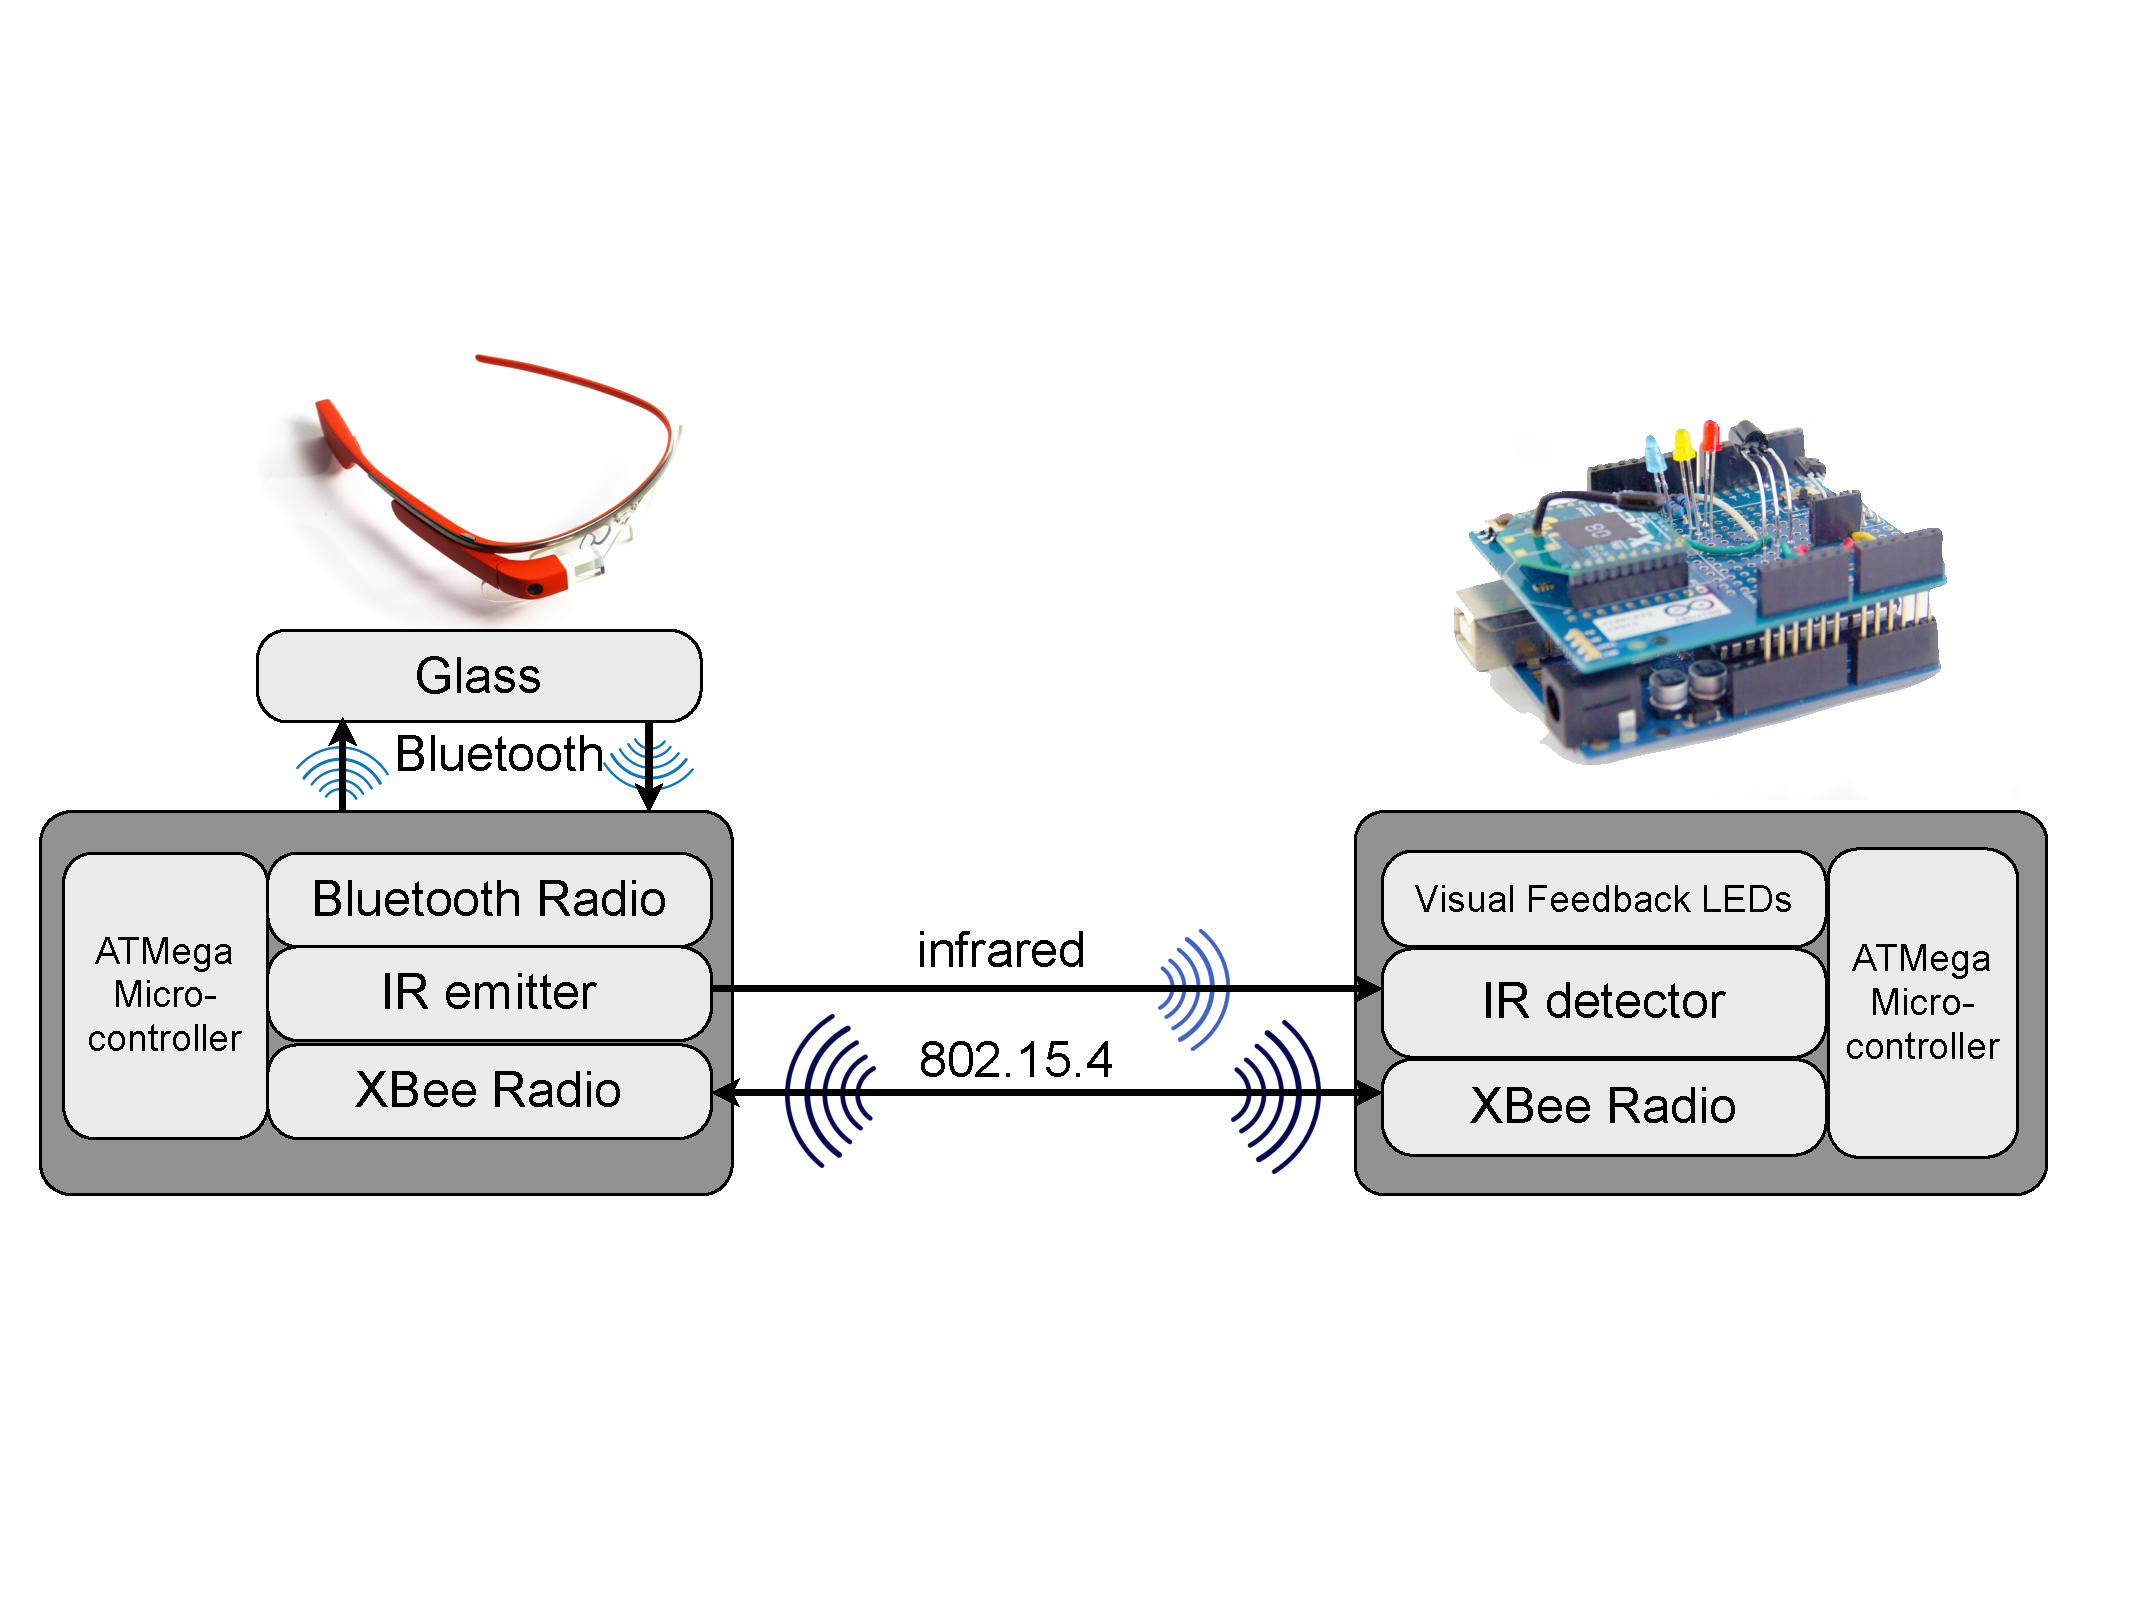
\includegraphics[width=0.95\columnwidth]{figures/architecture_new}
\caption{Our System architecture diagram. The selection is initiated through infrared but confirmed over 802.15.4.}
\label{fig:architecture}
\end{figure}

\newpage %bjoern hack fix
\subsection{Interaction Model}
From the user's perspective, interaction with \systemname proceeds in two stages (Figure~\ref{fig:interaction}): 


{\bf Scan:} The user first scans the environment to locate the position of the target. During this stage, Glass constantly sends out IR signals, and  targets offer immediate visual feedback when they receive a signal. The user confirms his desire to connect to a target by tapping on the Glass touchpad. Glass collects the responses from targets that have received IR reception through the backchannel of XBee. If there is only one single target in IR range, it is automatically selected. However, in a dense environment where multiple targets are within range, the user needs to refine his selection.


{\bf Refine:} When disambiguation is needed, the user must make an explicit selection among the targets within their view range. We have designed multiple refinement mechanisms -- all of which enable the user to select one from a subset of targets. The user confirms the current selection with a tap. Since the purpose of this stage is to disambiguate among potential targets, we will also use {\em disambiguation} to refer to this stage. Finally, a tap confirms a decision.


\begin{figure}[t!]
\centering
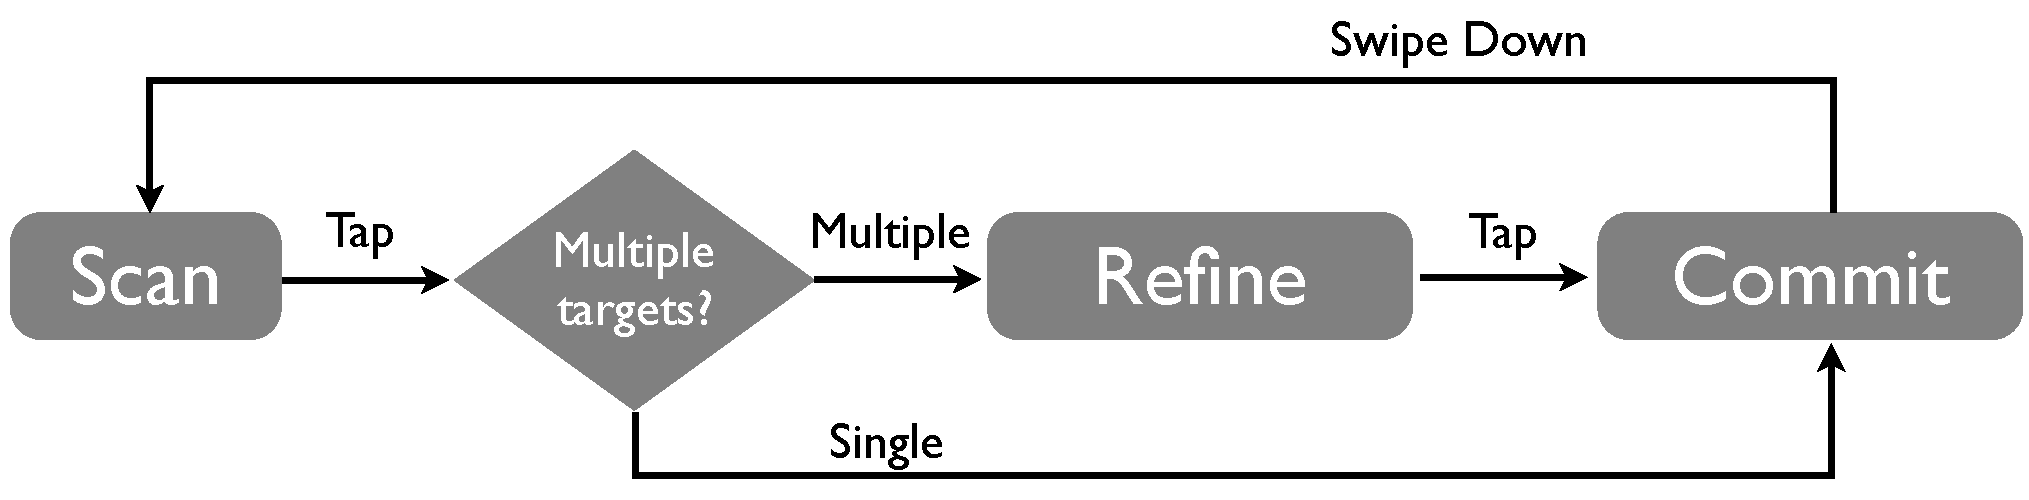
\includegraphics[width=\columnwidth]{figures/interactionModel2.pdf}
\caption{{\em scan} and {\em refine} -- two main stages during the interaction with HOBS. For completeness, we have also added the final state of {\em commit}.} 
\label{fig:interaction}
\end{figure}

The overall target acquisition time thus depends on scan and refine times, the probability that refinement is needed, and the time to commit an action (tap):
\begin{equation}
t_{total}=t_{scan}+P(refine)*t_{refine}+t_{commit}
\label{eq:time}
\end{equation}

In the following sections, we describe our iterative design and evaluation process to minimize the overall target selection time.

%%% Local Variables: 
%%% mode: latex
%%% TeX-master: "uist14"
%%% End: 

%!TEX root = uist14.tex

\section{Iteration 1: Naive IR}
\subsection{Problem Statement and Goal}
Our initial research question is: {\em Can IR-based targeting reduce the selection time compared to the case where only UI list navigation is used on a head-worn device?} 

\subsection{Technique}
In our first implementation, we use IR for scanning as described in the previous section. For the refinement technique, we simply show a list of the subset of targets that have received IR signals on the Glass display. Since we only know that the targets are within the range of users' head orientation. We order them using their ids; and in realistic environment target names can also be used if names can be assigned. We then let users swipe to select from that list and tap to confirm the intended target.

A natural point of comparison is an interface that does not use any head orientation information - it always shows a complete list of all targets. We implemented a list view where users swiped forwards and backwards on the Glass touchpad to navigate incrementally through the list. To quantify the benefit of using IR for the scanning step, we carried out a target acquisition study which compares the {\em Naive IR selection} and {\em list selection}.  

\subsection{Method}
We deployed 10 wireless nodes in an indoor environment (Figure~\ref{fig:targeting-study-layout}). Each of them has a number as ID and a letter representing the name. We recruited 14 participants from our institution for this study. 13 had never used Glass before, so we offered a Google Glass tutorial before the experiment for them to get familiar with Glass gestures. Four participants wore prescription glasses, which may have affected their task performance as wearing glasses beneath Glass makes it more cumbersome to secure the position of Glass and to adjust the screen to the optimal angle. In this study, the IR LED was fixed and not repositionable as shown in Figure~\ref{fig:glass}.

\begin{figure}[t]
\centering
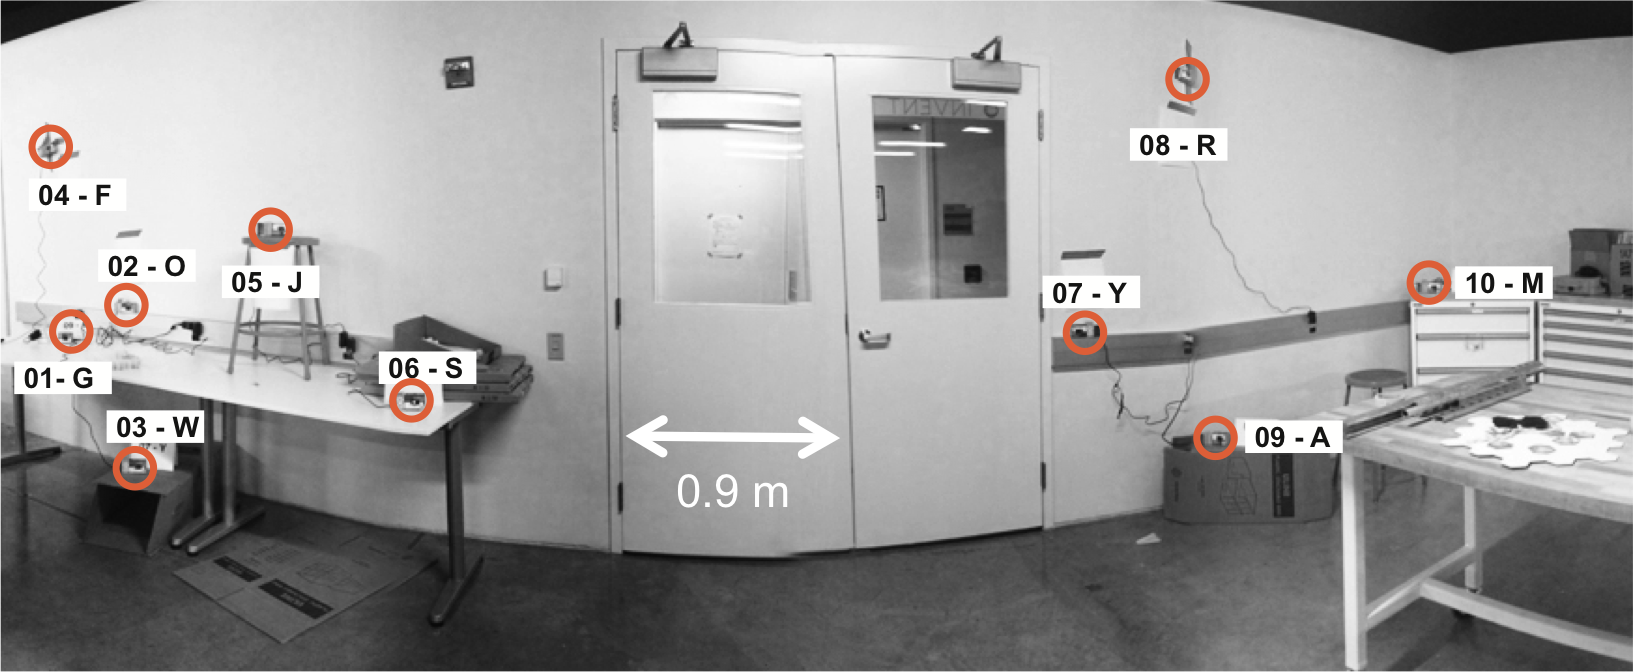
\includegraphics[width=1.0\columnwidth]{figures/study-layout1.png}
\caption{In the targeting study, participants were asked to find and select one of 10 targets in the lab environment.}
\label{fig:targeting-study-layout}
\end{figure}

In the within-subject study, half of the participants performed {\em IR selection} first and the other half used {\em list selection} first. For each selection condition, we conducted 15 target selection by randomly choosing from all the targets. During the study, we measured the {\bf target acquisition time} for each target selection. Afterwards, participants were asked to complete a survey that is mainly open-ended answers about their experience.

%% remove this for now
%% Our measurements suggest that IR communication can be targeted to an area about 60-120cm in diameter, up to 5m in front of the user. These values are a reasonable match for selecting targets in a room-size environment. A wider beam would lead to an increased chance of multiple appliances receiving IR signals simultaneously. A narrower beam will make targeting more challenging, given the precision constraints of human head movement.

\subsection{Results}

\begin{figure}[t]
\centering
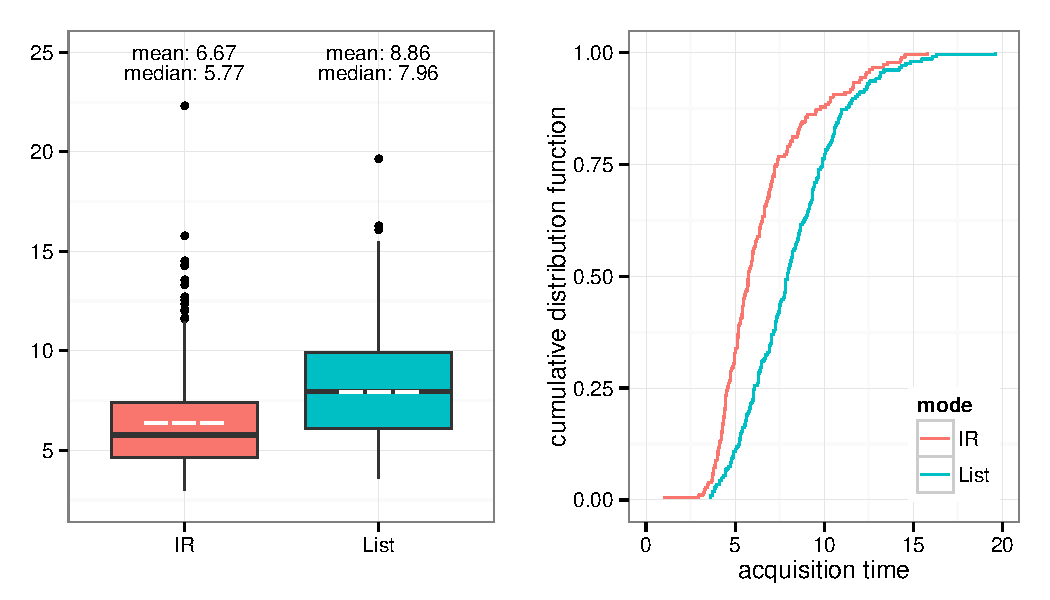
\includegraphics[width=1.0\columnwidth]{figures/result_study1a.pdf}
\caption{Boxplot of target acquisition time for {\em IR selection} and {\em list selectioN} is shown on the left. The center of each box is the median value, while we annotate the mean value using white dashed lines.}
\label{fig:ir_vs_list}
\end{figure}

\begin{figure}[t]
\centering
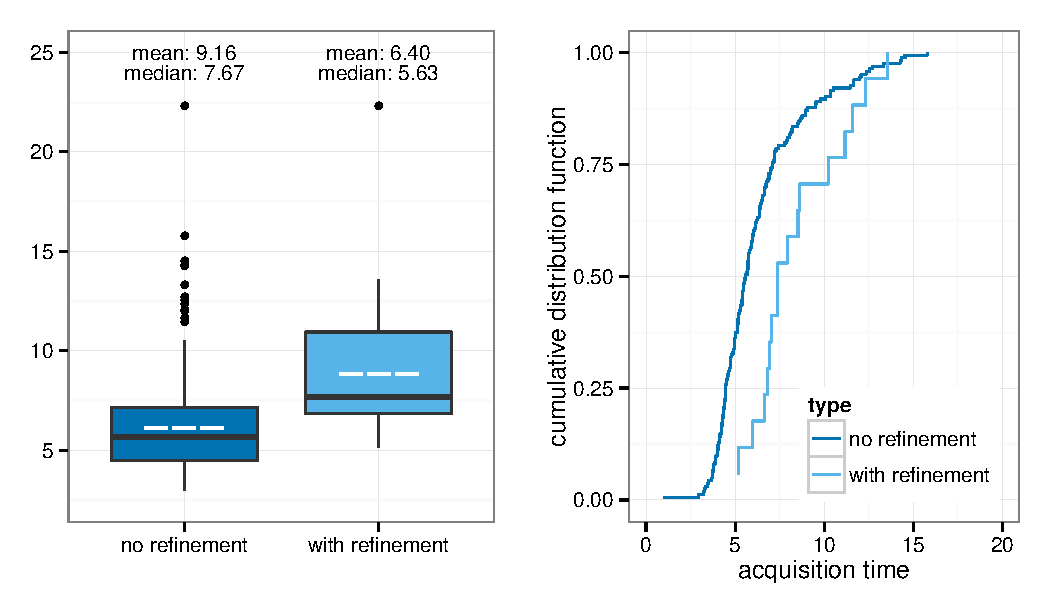
\includegraphics[width=1.09\columnwidth]{figures/result_study1b.pdf}
\caption{Boxplot and CDF of target acquisition time when refinement is needed or not in {\em IR selection}}.
\label{fig:with_without_refinement}
\end{figure}

\begin{figure}[t]
\centering
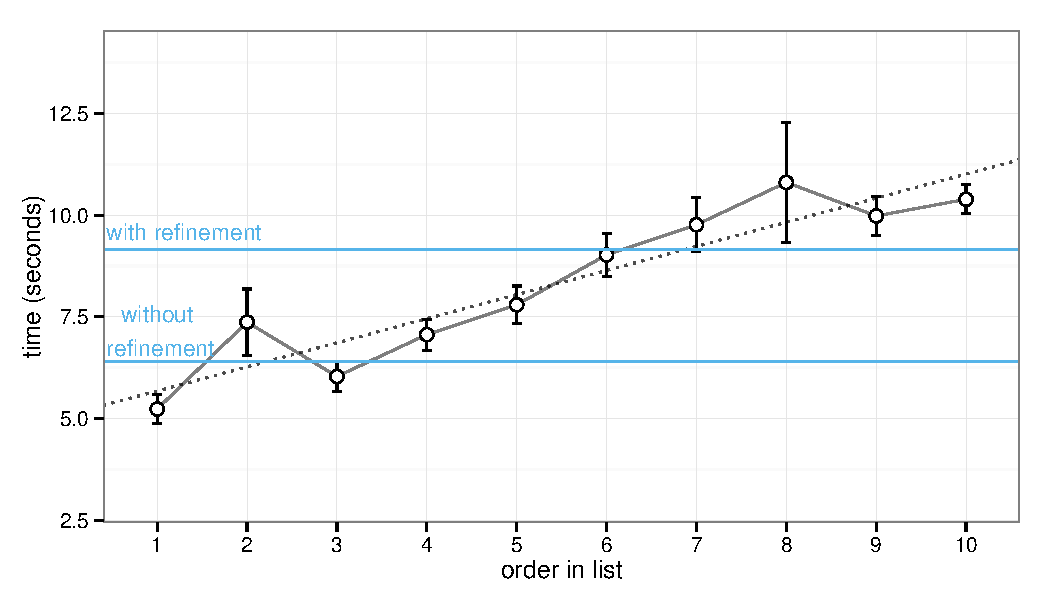
\includegraphics[width=1.0\columnwidth]{figures/result_study1c.pdf}
\caption{Times taken to select a device vs.~its order in the {\em list selection}. The dotted line is a linear fit between the average time and target orders in the list. Two horizontal solid lines are the average target acquisition times in {\em Naive IR} when refinement is needed or not.}
\label{fig:time-vs-list-order}
\end{figure}

Our results indicate that {\em IR selection} outperforms {\em list selection}.  The average target acquisition time for {\em IR selection} is 6.67 seconds 
while {\em list selection} took 8.86 {\em list selection also requires visual search, I think...} seconds (see Figure~\ref{fig:ir_vs_list}). Student's t-test shows a significant difference ($t(279)=-3.81, p=0.00017$).

To understand how scanning and refinement contribute to total selection time, we split the data from {\em IR selection} into two parts -- trials that required refinement and ones that did not. It takes 6.40 seconds (on average) to complete  a selection without any refinement, but 9.16 seconds with refinement, indicating that an additional 2.76 seconds are needed for disambiguation (see Figure~\ref{fig:with_without_refinement}). This difference is significant ($t(19)=-2.7827, p=0.012)$ using t-test.
%  \bjoern{I don't understand why we have 279 DF in the previous test but only 19 here??}). 
%% \ben{Because the times when refinement is needed is only 18 times, so the DF is bounded by the samples.}
Because many targets were spaced far apart, refinements were only necessary in 10\% of total {\em IR selection} trials in this study.

To further generalize the results, in Figure~\ref{fig:time-vs-list-order}, we show the acquisition time for each individual target in {\em list selection} condition, ordered by their relative position in the list. Since with IR technique, the acquisition time is invariant from each target's order, we use solid lines to represent the average performance of {\em IR selection}. From this figure, we can see that once there are more than 6 targets, the average acquistion time will be larger than IR selection, even if disambiguation is needed. %Therefore, we argue that once there are more targets in the physical space, the {\em list selection} method is not scalable. Further more, in real-life scenarios, targets would have longer names than an alphabet letter. This would increase the searching and text comparison time and also reduce the number of targets being shown in the UI screen.

As for the qualitative feedback, 11 out of 14 participants preferred IR selection over list mode (two preferred list, one was undecided). While both interfaces were judged similarly on overall ease of connecting, list selection was perceived to be cumbersome. One user noted benefit of {\em IR selection} being \studyquote{more direct [than list mode]}, allowing users to focus on the targeted objects instead of the screen. One subject called it \studyquote{natural to interact with things just by looking at them}. Another mentioned that \studyquote{it's really convenient that what I'm looking at is what I'm targeting}, and many participants compared the overall time of target acquistion. One subject pointed out that \studyquote{{\em IR selection} doesn't requires you to swipe a lot of times like list mode but list selection}.

In summary, {\em Naive IR} can outperform linear list selection, and most users like this head-orientation based targeting. But from our quantified study result, the refinement step detracts significantly from the efficiency of the technique.


% learned that with IR, we can have effectively reduced the overall target acquisition time. And the major gain comes from the fact that {\em coarse selection} helps reduce the chances of entering {\em fine selection} stage.

%\subsubsection{Preference}

%Eleven of 14 users preferred infrared mode over list mode (three preferred list, one was undecided). While both interfaces were judged similarly on overall ease of connecting, list navigation was also perceived to be cumbersome. As self-report data can easily skew positive as participants try to please experimenters, we also asked participants to elucidate why they preferred one interface over the other.

%List mode had certain advantages: It was judged to be more accurate and predictable as there was always exactly one device selected in the list (\studyquote{With the list you never have to worry about accidentally picking up two targets}). Also, it did not require a clear line of sight to the target device so participants did not have to move from their starting position (\studyquote{The shortcoming of the IR mode was that you had to be a certain distance away in order for it to detect the appliance}). 

%On the other hand, list mode was judged to be more \studyquote{annoying} and tedious. The temple-based touchpad for selection was difficult to use for a participant with long hair: \studyquote{List mode was physically difficult for me to navigate, since my long hair wasn't tied back and it kept interfering with my swiping.} Another participant also commented on the ergonomic challenge of touchpad use on Glass: \studyquote{The strength of the IR mode was that I didn't have to use my fingers as much to control. If the items were spaced relatively far apart, it was easy to select a specific appliance.}

%One noted benefit of infrared mode was a feeling that it was \studyquote{more direct [than list mode]}, allowing users to focus on the targeted objects instead of the screen. One subject called it \studyquote{natural to interact with things just by looking at them}. Another mentioned that \studyquote{it's really convenient that what I'm looking at is what I'm targeting}. 

%A few perceived weaknesses of infrared mode were the necessity to move the head in order to control a device and the imperfect mapping of gaze to target. One participant said that it was \studyquote{awkward to be aiming your head at things, tweaking back and forth to get it right}. Another noted that observing the head movement didn't capture the site of her attention, because \studyquote {eye movement is an important part of how people look around}. Users had to learn the usable angle of the IR emitter before they became successful at controlling the devices: \studyquote{I had to compensate by tilting my head up a little bit.}

%%% Local Variables: 
%%% mode: latex
%%% TeX-master: "uist14"
%%% End: 

%!TEX root = uist14.tex

\section{Iteration 2: Intensity IR}

%With our first study, we learn that using IR to perform {\em coarse selection} can reduce the overall target selection time. A major reason for the improvement is because disambiguation is only needed 10\% of the time. 
%because in many cases there will be only one target in range and fine selection is not needed, and in cases where it’s needed, the list length has been effectively reduced. 

Performance of the {\em Naive IR} technique will degrade as target density in an environment increases, as increased density will require refinement steps. We therefore ask a follow-up research question: {\em How might we improve selection time in a dense environment?}

\subsection{Technique}
Previously we only used IR reception as a binary signal for identifying potential targets. We hypothesize that IR intensity at the receiver side can provide more information about the likelihood that a user intended to select a particular target. Received IR intensity falls off with distance between IR emitter and receiver as well as with the angle between the emitter and receiver. To measure intensity, we add an IR light-to-voltage converter TSL267-LF by AMS-TAOS USA Inc.

% transmitter webpage: http://www.digikey.com/product-search/en?x=0&y=0&lang=en&site=us&KeyWords=475-2919-ND
% http://www.digikey.com/product-detail/en/TSL267-LF/TSL267-LF-ND/3095052

We have empirically measured the intensity distribution at the receiver for this configuration in Figure~\ref{fig:measurement}. Our measurements confirm that angular difference has a large effect on the intensity readings (see how the IR intensity distribution changes when the \changes{angle has increased}) \achal{this sounds awkward to me - maybe "Note the changes in IR intensity distribution when the angle increases}.

\begin{figure}[t]
\centering
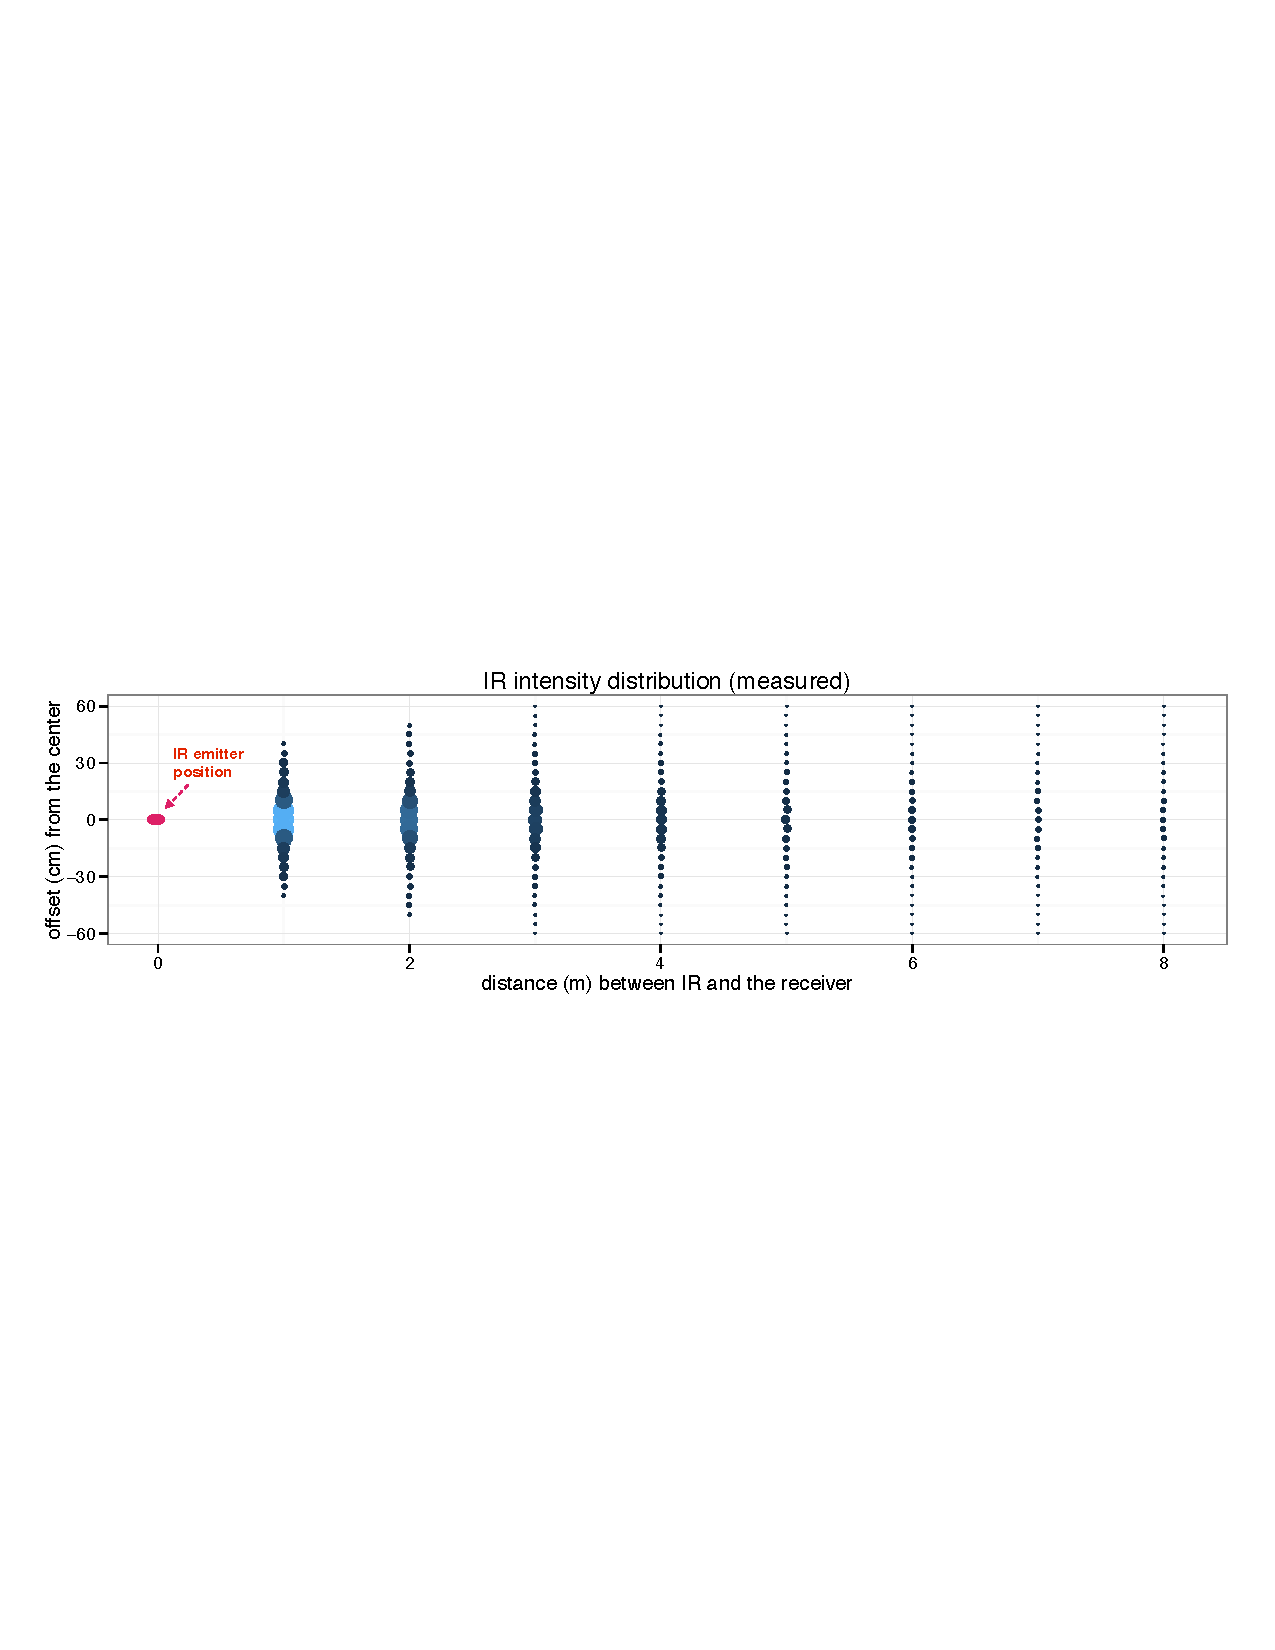
\includegraphics[width=0.95\columnwidth]{figures/IRIntensityDistribution.pdf}
\caption{This figure shows an empirical measurement of IR intensity at different positions. We measure the intensity at a plane every meter away from the IR emitter. On that plane, a sample is taken every 5 centimeters, \changes{and we stop when the reading is smaller than ambient noise.} \changes{To match our assumption about the relationship between angles and intensities, the vertical axis is changed to the degree of the angle.} The size and color brightness represent the intensity of the readings for visualization.}
\label{fig:measurement}
\end{figure}

The intensity information is used in two ways:
\begin{enumerate}
\item When multiple targets have received IR signals and reported the intensity readings, we discard those whose intensities are significantly lower than the largest reading\footnote{In our current implementation, we empirically set it to be half of the ADC resolution, which is frequently used as it indicates a 3dB loss in the signal strength.}. Therefore, when there is only one target within the line of sight, the IR intensity approach has the same behavior as the previous iteration - no disambiguation is needed. When the environment becomes more populated, the new design can filter some peripheral targets out, reducing $P(refine)$, the likelihood of entering the refinement stage.
\item When refinement is still needed, meaning that multiple targets have relatively close intensity values, the system sorts the disambiguation list according to the IR intensity, from strongest to weakest. We hypothesize that this will reduce $t_{refine}$ significantly by minimizing extra navigation steps, as the first list item will generally match the intended target.
\end{enumerate}

\subsection{Method}
To quantify the improvement in this design we performed a second study to compare the {\em Naive IR} and {\em Intensity IR} approaches. Because we were interested in discovering performance differences in denser environment, we re-positioned the 10 nodes and set them up in a smaller area (see Figure~\ref{fig:study-layout2}). We recruited 10 participants for this study. Each  user performed 30 target acquisition tasks for each approach. \sean{Need to add desciption about participants physical movements or restrictions here. Ben or Claire?} As in our first within-subject study, half of them perform {\em Naive IR} first and the other half {\em Intensity IR} first.

\begin{figure}[t]
\centering
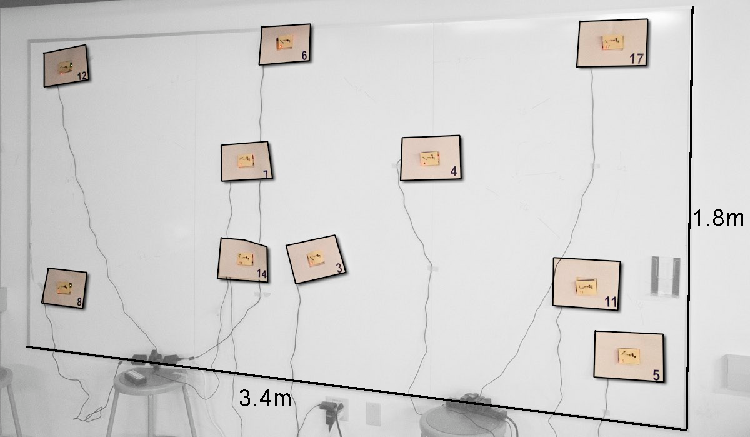
\includegraphics[width=0.95\columnwidth]{figures/study-layout2.pdf}
\caption{The environment setup for our second study. In comparison to our first study, we have deliberately increased the target density.}
\label{fig:study-layout2}
\end{figure}

% new study results
% ceiling(c(nrow(name), nrow(name_multiple), wrong_guess, wrong_percentage * 100))
% intensity
%  300 167  74  45
% name
%  300 225 145  65

%% first one
%% 
%             Outcome 1	Outcome 2	     Total
% Group 1 	167	133	300
% Group 2	225	75	300
% Total	        392	208	600
%% Chi squared equals 24.755 with 1 degrees of freedom. 
%%  The two-tailed P value is less than 0.0001


% 	    Outcome 1	Outcome 2	     Total
% Group 1	74	93	167
% Group 2	145	80	225
% Total	        219	173	392
% Chi squared equals 15.758 with 1 degrees of freedom. 
%   The two-tailed P value is less than 0.0001




\subsection{Results}
{\em Intensity IR} reduces the number of trials in which refinement dialogs are needed from 225 of 300 in {\em Naive IR} to 167 of 300 trials. A Chi-square test shows this difference is significant ($\chi^2(1) = 24.755$, \changes{$p < 0.001$}). This demonstrates that the new approach successfully reduces the probability that a disambiguation dialog is needed.

In the cases where disambiguation is inevitable, {\em Intensity IR} sorts the list based on the intensity reading, while {\em Naive IR} sorts alphabetically. {\em Intensity IR} reduces the fraction of refinement trails in which additional list navigation is necessary (i.e., the first, already selected element is incorrect).  {\em Intensity IR} sorted the desired target as the first one in the list in 55\% of cases (93 of 167). In comparison, for {\em Naive IR}, only 35\% of trials sorted the desired target as the first one in the list (80 out of 225). A Chi-square test show that this difference is significant (with $\chi^2(1) = 15.758$, \changes{$p < 0.001$}).

From Figure~\ref{fig:study2}, we can see that the overall target acquisition time has decreased from 4.31 seconds for {\em Naive IR} to 3.64 second for {\em Intensity IR}. This difference is also significant ($t(555)=3.2945$, $p=0.001$).

%  t.test(name$complete, intensity$complete)

% 	Welch Two Sample t-test

% data:  name$complete and intensity$complete
% t = 3.2945, df = 555.272, p-value = 0.001049
% alternative hypothesis: true difference in means is not equal to 0
% 95 percent confidence interval:
%  0.2707875 1.0704747
% sample estimates:
% mean of x mean of y 
%  4.311340  3.640709 

\begin{figure}[t]
\centering
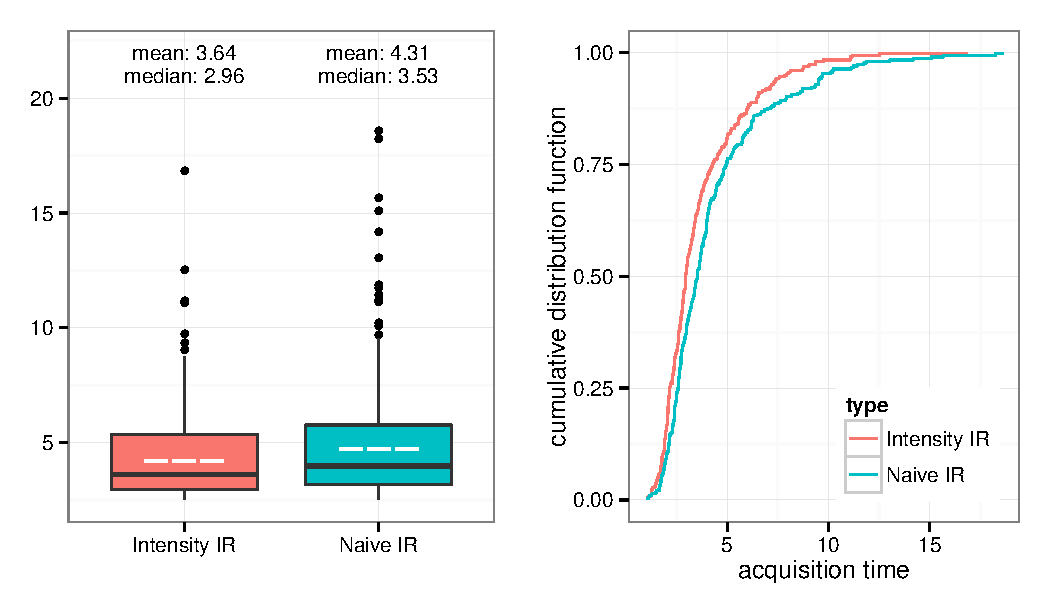
\includegraphics[width=0.95\columnwidth]{figures/result_study2.pdf}
\caption{Boxplot and CDF of the target acquisition time in {\em Naive IR} and {\em Intensity IR} conditions.}
\label{fig:study2}
\end{figure}

\sean{If possible, add how we observed participants physical movements in this iteration. Better if we can compare to i1.} One side effect that we have observed in this approach is that the {\em Intensity IR} sometimes eliminates the desired target during the {\em scanning} stage. Out of 300 trials, \changes{the target was accidentally eliminated in 13 (4.3\%).} This is higher than the error rate for {\em Naive IR} (5 out of 300, ~1.6\%). \changes{Even though the higher error rate increases the chance of multiple attempts in target selection, our analysis above illustrates that overall performance of {\em Intensity IR} is still better than {\em Naive IR}. }  % but this is the trade-off for the overall faster acquisition time.

%%% Local Variables: 
%%% mode: latex
%%% TeX-master: "uist14"
%%% End: 

\subsection{Technique}

We introduce a third technique that uses a combination of motion sensors and IR to learn the relative orientations of
targets in a room and intelligently suggest targets during refinement (see
Figure~\ref{fig:third_technique}).

This absolute orientation cannot be applied to all indoor
environments, since the user’s movements through the space could change the relationships between targets. However, with the constraint that the targets are spread around the periphery, their relative orientations are stable
(see Figure~\ref{fig:third_principle}). 

\begin{figure}[t]
\centering
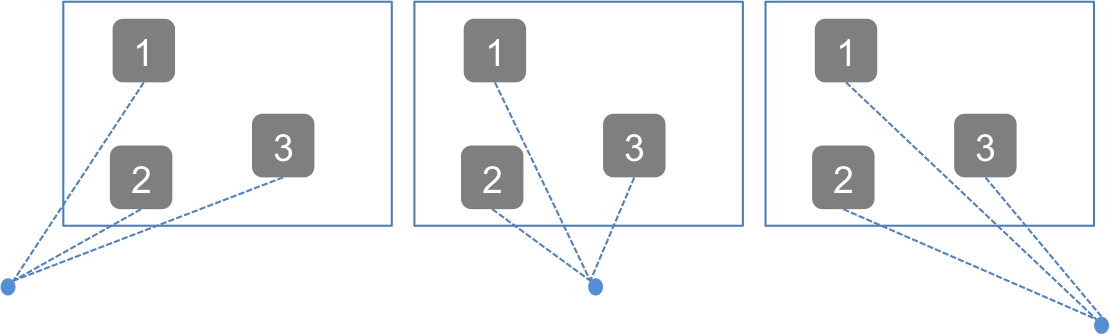
\includegraphics[width=1\columnwidth]{figures/third_principle.png}
\caption{Even when the user's absolution position changes, the relative relationship in the orientation space remain invariant.}
\label{fig:third_principle}
\end{figure}

\begin{figure}[t]
\centering
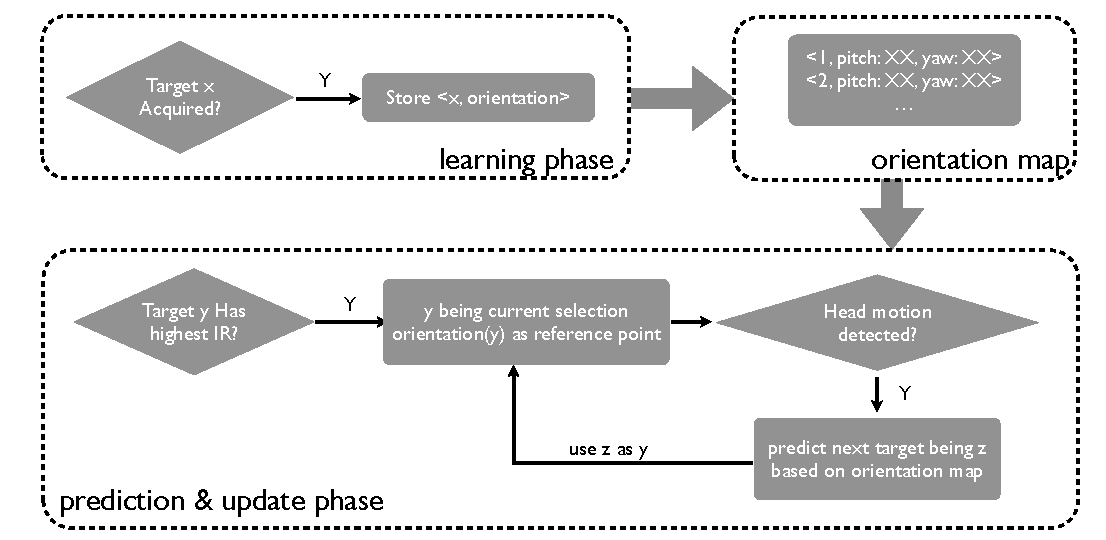
\includegraphics[width=1\columnwidth]{figures/third_technique3.pdf}
\caption{\ben{figure in interactionModel2.key file.} Our third technique learned each target's absolute orientation and construct the orientation map. Though we store the absolute orientation value, during the {\em refinement} stage, the prediction is only based on relative changes to a reference point. In such a way, the prediction will work regardless of user's position.}
\label{fig:third_technique}
\end{figure}

In the learning stage, the user scans over the targets, and the
system attains the absolute orientation of each device from IR and motion sensors. From this information it can abstract out their relative positions and build an {\em adjacency map}.

After the map is created, the user can hold down on the touchpad to enter a
quasi-mode for refinement. In this quasi-mode, one device lights up at a time. When the user turns his head in the direction of another device, the light switches to that device. Therefore, the user can move between devices one at a time with slight head movements. We implement this interaction by calculating the user's direction of motion using a low-passed history of sensor measurements and searching through the adjacency map for
the nearest device in that direction. 

\subsection{Evaluation}
We evaluate the head motion refinement method by holding an informal study and collecting qualitative feedback from a subset of 4 users from the Iteration 2 study. In the study, we asked users to try cycling through the targets using the new quasi-mode.
The users had strong preferences for the new method of refinement. On a scale from 1-7, 1 being the least mental effort and 7 being the most mental effort users rated the old technique 4.25 and the new technique 2 on average. 100\% indicated a preference for head movement to list navigation. One user referenced the issue of naming targets that the list necessitates, preferring the experience of ``matching visual cues rather than numbers''. Another participant remarked that it ``just made more sense'' and was a ``more natural way for demonstrating intentionality.'' The users prefered the new mapping in relation to the whole environment: ``it leveraged the spatial sense that I already had just by using the system''. They were also delighted to avoid list navigation, which they now called ``difficult'' and ``painful''. 
%\section{Disambiguation Techniques}
\label{sec:disamb-techn}

This section discusses the three different disambiguation techniques we have proposed.

\subsection{Using IR Intensity}
\label{sec:using-ir-intensity}

\subsection{Using Glass Sensors}
\label{sec:using-glass-sensors}

\subsection{Manual Disambiguation}
\label{sec:manu-disamb}



%%% Local Variables: 
%%% mode: latex
%%% TeX-master: "uist14"
%%% End: 

%
\section{Evaluation}
\label{sec:evaluation}

This section we present our work on the evaluation and user study.


%%% Local Variables: 
%%% mode: latex
%%% TeX-master: "uist14"
%%% End: 


%% the rest of the paper seems to be fine; it's mainly the texts
\section{Applications}
\label{sec:applications}

In this section we describe four possible applications that can be built on top of the head orientation-based selection. We focus our discussion on the ``universal remote control'' system. 

%%% Local Variables: 
%%% mode: latex
%%% TeX-master: "uist14"
%%% End: 


\section{Discussion}
\label{sec:discussion}

We discuss a few issues with the system.
%%% Local Variables: 
%%% mode: latex
%%% TeX-master: "uist14"
%%% End: 

\section{Conclusion}
We introduced a novel method for selecting and controlling smart appliances in physical spaces through  infrared targeting based on head orientation. The design takes advantage of the fact that visual attention can express intention, makes it ituitive and helps users remain their focus in the physical world. It addresses the naming and scaling challenges faced by handheld mobile devices. While we present a prototype approach that requires that the user carry additional hardware, all parts can readily be miniaturized and integrated into future head-worn hardware. We also introduced a disambiguation technique in case head orientation is not sufficient to determine a unique target. We characterized our devices performance, arguing that it is matched well to the amount of head movement people can control without strain. A target acquisition study showed that the technique is efficient; a home control scenario showed promise but also limitations when trying to control complex appliances. As our environment continues to be populated by a swarm of sensing and actuation devices, methods to interrogate and control our smart environments may become increasingly important.
%\section{Acknowledgments}
%We thank our user study participants and the a

\iftoggle{anonymous}{
% no acks in anonymous submission
}{
  \section{Acknowledgments}
  
  This work was supported in part by the TerraSwarm Research Center, one of six centers supported by the STARnet phase of the Focus Center Research Program (FCRP) a Semiconductor Research Corporation program sponsored by MARCO and DARPA. Additional support was provided by a Sloan Foundation Fellowship and a Google Research Award.
}
%figure template:
%\begin{figure}[!h]
%\centering
%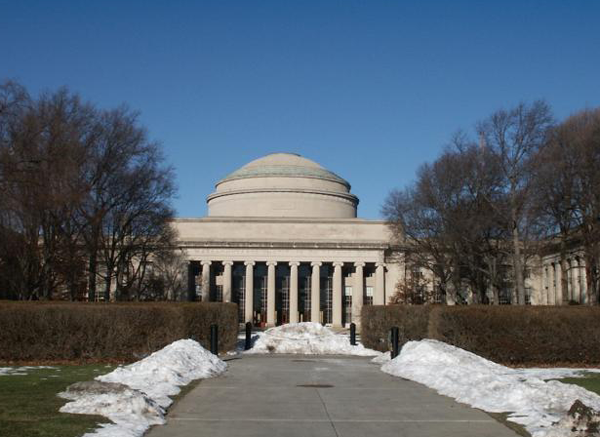
\includegraphics[width=1.0\columnwidth]{Figure1}
%\caption{With Caption Below, be sure to have a good resolution image
%  (see item D within the preparation instructions).}
%\label{fig:figure1}
%\end{figure}

% Balancing columns in a ref list is a bit of a pain because you
% either use a hack like flushend or balance, or manually insert
% a column break.  http://www.tex.ac.uk/cgi-bin/texfaq2html?label=balance
% multicols doesn't work because we're already in two-column mode,
% and flushend isn't awesome, so I choose balance.  See this
% for more info: http://cs.brown.edu/system/software/latex/doc/balance.pdf
%
% Note that in a perfect world balance wants to be in the first
% column of the last page.
%
% If balance doesn't work for you, you can remove that and
% hard-code a column break into the bbl file right before you
% submit:
%
% http://stackoverflow.com/questions/2149854/how-to-manually-equalize-columns-
% in-an-ieee-paper-if-using-bibtex
%
% Or, just remove \balance and give up on balancing the last page.
%
%% \balance

\bibliographystyle{acm-sigchi}
\bibliography{sui14}
\end{document}
